% Copyright (c) 2008-2009 solvethis
% Copyright (c) 2010-2016,2018-2019,2022 Casper Ti. Vector
% Copyright (c) 2021 Kurapica
% Copyright (c) 2022 iofu728
% Overleaf version.

%*********************************************************************
% pkuthss_zyz: 北京大学研究生学位论文模板_ZYZ修改及使用心得
% 2024/06/15
%
% 重要提示:
%   1. 当前模板基于pkuthss v1.9.2,也参考了pkuthss v1.9.2和北京大学工学院的LaTex模板
%   2. 当前overleaf版符合研究生学位论文要求,可通过图书馆审核
%   3. 请使用UTF-8编码,XeLaTeX方式编译
%   4. 请仔细阅读用户文档
%   5. 修改、使用、发布本文档类请务必遵循LaTeX Project Public License和知识共享4.0
%   6. 感谢github作者 @iofu728 @zhiyunyao 提供了非常漂亮的pkuthss模板
%*********************************************************************

%*********************************************************************

%*********************************************************************

\documentclass[UTF8,fontset=fandol,ugly,language=chinese]{pkuthss}
  % 学位论文模式  ugly    (默认打开,请保留)
  % 盲审模式     blind   (默认关闭)
  % 语言        language (默认chinese | english)
  % 字体库       fontset
  %   auto | windows | windows@overleaf | mac | fandol | ubuntu | none
  % windows*, mac为商业字体,如需使用请遵循相应版权协议(默认下overleaf中不可用)
  % fandol与windows效果相近,但字符库偏少,推荐使用(默认);
  % ubuntu字体效果偏差较大; 设为none时需自行配置字体集;


% --- 参考文献遵循GB/T 7714-2015标准,使用biblatex-gb7714-2015 宏包。 ---
% 1.此处使用顺序编码制 gb7714-2015
%%% \usepackage[backend=biber, style=gb7714-2005]{biblatex}
% \usepackage[backend=biber, style=gb7714-2015, gbnamefmt=lowercase]{biblatex}
% 2.此处使用著者-出版年制则 gb7714-2015ay。
%   使用 著者-出版年制 (添加了许多选项以调整引用格式、字体、文献排版顺序等,请自行参考GB/T 7714-2015标准biblatex 宏包的说明文档了解选项内容)
 \usepackage[backend = biber, style = gb7714-2015ay, gbnamefmt=familyahead, gbtype=false, maxcitenames=2, mincitenames=1, uniquelist=false, gbcitelabel=parensqj]{biblatex}
 \DefineBibliographyStrings{english}{
 andincite = { and }, %判断为英文文献时两个作者使用 A and B 
 andincitecn = { 和 }, %判断为中文文献时两个作者使用 张三 和 李四 
 }
%\DeclareDelimFormat[textcite,citet, citep]{andothersdelim}{}%\space

% ------ ZYZ:设置英文断行不要断字 ------
\tolerance=1
\emergencystretch=\maxdimen
\hyphenpenalty=10000
\hbadness=10000

% 示例文档用包和设定,该段均可移除.
\usepackage{pdfpages}
\usepackage{enumitem,fancyvrb}
\usepackage{booktabs,multirow,longtable,makecell} % 表格相关
\RecustomVerbatimEnvironment{Verbatim}{Verbatim}{frame = single, tabsize = 4, fontsize=\footnotesize}
\renewcommand{\v}[1]{\boldsymbol{#1}}
\newcommand\pkg[1]{\textsf{#1}}

% 参考文献边距字体
\setlength{\bibitemsep}{3bp}
\renewcommand*{\bibfont}{\zihao{5}\linespread{1.27}\selectfont}

%自定义
\newcommand{\old}[1]{\textcolor{blue}{\sout{#1}}}
\newcommand{\new}[1]{\textcolor{red}{#1}}

\pkuthssinfo{
    cthesisname = {博士学位论文},
    thesiscover = {博士研究生学位论文},
    ethesisname = {Doctor Thesis},
    ctitle = {北京大学博士论文模板 zyz版},
    etitle = {pkuthss\_zyz},
    cauthor = {ZYZ先生}, eauthor = {Mr. ZYZ},
    studentid = {4367497427},
    % 具体时间以教务为准,初稿3月,送审4月,答辩5月,最终6月。
    date = {\zhdigits{2024}\ \ 年\ \ \zhnumber{6}\ \ 月}, % June, 2022
    school = {学院名},
    cmajor = {二级学科}, emajor = {major},
    direction = {研究方向},
    mentorlines = {1}, % 导师个数
    % 副教授 A.P. 讲师 Lec. 教授 Prof.
    cmentor = {导师姓名\ \ 职称}, ementor = {Prof.\ Name},
    ckeywords = {博士论文,北大,模板},
    ekeywords = {PhD Thesis, Peking University, Template},
    % 盲审模式参数, 需在documentclass增加blind
    blindid = {XXXXXXXXX}, discipline = {XXXX}
}
\addbibresource{ref.bib}


\begin{document}
    \frontmatter
    \pagestyle{empty}
    \maketitle
    \cleardoublepage
    % 需替换门户版权声明pdf
   % Copyright (c) 2008-2009 solvethis
% Copyright (c) 2010-2017,2021 Casper Ti. Vector
% Copyright (c) 2021 iofu728
% All rights reserved.
%
% Redistribution and use in source and binary forms, with or without
% modification, are permitted provided that the following conditions are
% met:
%
% * Redistributions of source code must retain the above copyright notice,
%   this list of conditions and the following disclaimer.
% * Redistributions in binary form must reproduce the above copyright
%   notice, this list of conditions and the following disclaimer in the
%   documentation and/or other materials provided with the distribution.
% * Neither the name of Peking University nor the names of its contributors
%   may be used to endorse or promote products derived from this software
%   without specific prior written permission.
%
% THIS SOFTWARE IS PROVIDED BY THE COPYRIGHT HOLDERS AND CONTRIBUTORS "AS
% IS" AND ANY EXPRESS OR IMPLIED WARRANTIES, INCLUDING, BUT NOT LIMITED TO,
% THE IMPLIED WARRANTIES OF MERCHANTABILITY AND FITNESS FOR A PARTICULAR
% PURPOSE ARE DISCLAIMED. IN NO EVENT SHALL THE COPYRIGHT HOLDER OR
% CONTRIBUTORS BE LIABLE FOR ANY DIRECT, INDIRECT, INCIDENTAL, SPECIAL,
% EXEMPLARY, OR CONSEQUENTIAL DAMAGES (INCLUDING, BUT NOT LIMITED TO,
% PROCUREMENT OF SUBSTITUTE GOODS OR SERVICES; LOSS OF USE, DATA, OR
% PROFITS; OR BUSINESS INTERRUPTION) HOWEVER CAUSED AND ON ANY THEORY OF
% LIABILITY, WHETHER IN CONTRACT, STRICT LIABILITY, OR TORT (INCLUDING
% NEGLIGENCE OR OTHERWISE) ARISING IN ANY WAY OUT OF THE USE OF THIS
% SOFTWARE, EVEN IF ADVISED OF THE POSSIBILITY OF SUCH DAMAGE.


% 此处不用 \specialchap,因为学校要求目录不包括其自己及其之前的内容。
\chapter*{版权声明jjj}
% 综合学校的书面要求及 Word 模版来看,版权声明页不用加页眉、页脚。
\thispagestyle{empty}

任何收存和保管本论文各种版本的单位和个人hhh,
未经本论文作者同意,不得将本论文转借他人,
亦不得随意复制、抄录、拍照或以任何方式传播。
否则一旦引起有碍作者著作权之问题,将可能承担法律责任。

% 替换门户下载pdf
\begin{textblock}{1}(-0.8,-0.08)
    \colorbox{white}{
        
\includegraphics[height = 1.2448\textheight]{img/bqsm_example.pdf}
    }
\end{textblock}

% vim:ts=4:sw=4  
    \cleardoublepage
    \pagestyle{plain}
    \setcounter{page}{0}
    \pagenumbering{Roman}
   \begin{cabstract}
\addcontentsline{toc}{chapter}{摘要}

这里是摘要

\end{cabstract}

\begin{eabstract}
\addcontentsline{toc}{chapter}{ABSTRACT}

This is the abstract

\end{eabstract}

% vim:ts=4:sw=4

    \tableofcontents
    %% 如有需要插入表格索引、插图索引
    %\listoftables
    %\listoffigures
    %% 如有需要使用主要符号对照表
    %\begin{denotation}
\item[$x,y,m,n,t$] 标量,通常为变量
\item[$K,L,D,M,N,T$] 标量,通常为超参数
\item[$x\in \mathbb{R}^{D}$] D维列向量
\item[$(x_1,\cdots,x_D)$] D维行向量
\item[$(x_1,\cdots,x_D)^T$ or $(x_1;\cdots;x_D)^T$]  D维行向量
\item[$\v A\in \mathbb{R}^{K\times D}$]  大小为$K\times D$的矩阵
\item[$x\in \mathbb{R}^{KD}$]  ($KD$)维的向量
\item[$\mathbb{M}_i$ or $\mathbb{M}_i(\v x)$]  第$i$列为$\v 1$(或者$\v x$),其余为$\v 0$的矩阵
\item[$diag(\v x)$]  对角矩阵,其对角元素为$\v x$
\item[$\v I_N$ or $I$]  ($N\times N$)的单位阵
\item[$diag(\v A)$]  列向量,其元素为$\v A$的对角元素
\item[$\v A \in \mathbb{R}^{D_1\times D_2\times \cdots \times D_K}$]  大小为$D_1\times D_2\times \cdots \times D_K$的张量
\item[$\{x^{(n)}\}^{N}_{n=1}$]  集合
\item[$\{(x^{(n)},y^{(n)})\}^{N}_{n=1}$]  数据集
\item[$\mathcal{N}(\v x;\mu,\sum)$]  变量$x$服从均值为$\mu$,方差为$\sum$的高斯分布

\end{denotation}

    
    \mainmatter
    \chapter{引言}
\label{chap:introduction}

对论文写作而言,LaTex在公式图表的插入及引用、参考文献的引用和排版等方面相较word更为便捷,然而北京大学博士研究生学位论文的官方模板是以word形式发布的,未有官方的LaTex模板。本人进行论文写作时,找到一些符合北大博士论文要求的LaTex模板,主要是pkuthss系列和北京大学工学院的模板。

本模板主要以pkuthss v1.9.2为基础,也融合了工学院模板的一些优点,主要特点是对“著者-出版年制”的参考文献引用方式做了更具体的设置,较pkuthss v1.9.2原始模板更规范。本模板更像是本人使用pkuthss的经验总结,可以作为使用者的一种参考,模板中的一些缺点也将在后续章节说明。LaTex有许多使用技巧,使用者可根据需求搜索攻略,期待后来人能将该模板不断完善。

\section{参考模板}

提供三个北大博士学位论文的LaTex模板。

\begin{enumerate}[itemindent=0.3em]     % 用enumerate环境可能需要控制缩进量
    \item pkuthss v1.9.2:https://github.com/iofu728/pkuthss
    \item pkuthss v1.9.4:https://github.com/zhiyunyao/pkuthss/tree/lite。该模板发布于2024年4月,推荐使用这一最新模板,将本模板作为参考即可。
    \item 工学院模板:https://www.coe.pku.edu.cn/service/biyedb/11187.html。本模板中研究生成果页参考了该模板。
\end{enumerate}

\section{编译要求}

本模板仅支持UTF-8文件编码和XeLaTex编译。请确保所有文件为UTF-8编码,编译时请修改编译器为XeLaTex。

\section{环境配置}

\subsection{在VSCode使用}

在本地环境下进行写作,推荐使用VSCode。

环境配置:安装TeX Live(可能需要8G左右的空间),在VSCode中配置LaTex Workshop扩展。相关方法网上已有许多。

需要注意的是,如果已安装了其他Tex系统(比如CTEX),可能与TeX Live冲突,VSCode编译时可能优先选择其他系统。使用者可以先试一下能否编译成功,再决定是否安装Tex Live。如安装Tex Live后仍编译不成功,需要卸载有冲突的Tex系统。

使用模板:在GitHub上下载该项目的zip压缩包,解压后在VSCode中打开\texttt{main.tex},用XeLaTex编译即可。

\subsection{在overleaf使用}

如不想在进行本地环境配置,也可以选择overleaf进行在线写作,只需将本模板包的所有文件copy到新建的项目里,或将GitHub下载的zip包上传到oveleaf中,用XeLaTex编译\texttt{main.tex}即可。

需要注意的是,overleaf对编译超过20 s的项目要收费,必须开通会员才可使用。截止2024年6月,学生会员的价格是9 $\$$ /月。

本模板项目较小,编译时间暂不到20 s,如编译一篇学位论文则必然超过20 s。

\section{本文档行文结构}

本说明文档结构如下:

第\ref{chap:introduction}章将介绍几种北大学位论文LaTex模板,并介绍本模板的使用方法。

第\ref{chap:reference}章将介绍本模板中参考文献的引用和排版方式。

第\ref{chap:fig_tab}章将介绍图表的插入、引用方式及使用中的问题和技巧。

第\ref{chap:equation}章将介绍公式的插入、引用方式及使用中的问题和技巧。

第\ref{chap:problem}章将介绍本模板存在的一些问题。

    \chapter{参考文献排版}
\label{chap:reference}

参考文献的引用和排版可以采用“顺序编码制”或“著者-出版年制”,本模板均通过符合GB/T 7714-2015 标准的biblatex 参考文献宏包(以下简称7714宏包)实现,在\texttt{main.tex}文件中选择其中一种方式即可。“顺序编码制”排版规则简单,使用时需要调整的参数很少。使用“著者-出版年制”时,需要调整的参数较多。以下给出本模板对参考文献排版的设计,以及示例、问题和思考。

\section{本模板的设计}

本人写作时曾惊讶于7714宏包的强大,使用者请一定查阅7714宏包说明文档,即本模板提供的\texttt{biblatex-gb7714-2015.pdf}文件,以了解各种用法。该宏包的相关信息也可网上搜索得到。

本模板对“著者-出版年制”选项设置为\texttt{\string\usepackage[backend = biber, style = gb7714-2015ay, gbnamefmt=familyahead, gbtype=false, maxcitenames=2, mincitenames=1, uniquelist=false, gbcitelabel=parensqj]\{biblatex\}}。主要选项意义如下:

\begin{itemize}
    \item \texttt{gbnamefmt=familyahead}:排版时姓在前名在后,类似于APA的样式;
    \item \texttt{gbtype=false}:不输出文献类型标识符。
    \item \texttt{maxcitenames=2,mincitenames=1}:超过\texttt{maxcitenames}个作者的文献,只输出\texttt{mincitenames}个作者,并添加“et al.”或“等”。
    \item \texttt{uniquelist=false}:\texttt{uniquelist}用于正文中引用(标注)标签的作者列表控制(目的是消除歧义)。这里设置为\texttt{faluse}表示仅用一个作者作为文中的标注标签,如果遇到同姓作者同一年的文献,通过在年份后添加字母以区分。
    \item \texttt{gbcitelabel=parensqj}:标注标签由全角圆括号包围。由于引用时会出现大量括号,该设置的目的是使正文中不会出现英文、中文括号混用的现象。
    \item 增加了中文文献用“和”、英文文献用“and”连接人名的设置。
\end{itemize}

\section{示例}
\label{sec:ref_example}

我们以北大论文word模板中的一段文字进行参考文献的示例。修改\texttt{main.tex}中的参考文献排版方式,可以对比“著者-出版年制”和“顺序编码制”两种方式的参考文献排版方式。

\texttt{环境中黑炭(black carbon)气溶胶的主要来源包括各种化石燃料和生物质燃料的不完全燃烧过程\cite{Penner1993,Bond2004},这些不完全燃烧在自然界和人类活动中都会发生,因此,环境中黑炭气溶胶的来源十分广泛。对当今大气环境中的黑炭,其主要来源是人类相关的燃料燃烧活动\cite{段凤魁_2007},此外,一些自然过程也会产生黑炭,如森林火灾、草原火灾等。根据过去的排放清单研究,大气环境中黑炭气溶胶的来源主要包括:1)有机燃料的燃烧,主要包括能源行业、工业部门、交通运输行业、居民生活中煤、石油、天然气和各种生物质燃料的使用。通常而言,燃烧效率越高,产生的黑炭气溶胶的量越低;2)工业炼焦,主要包括炼焦过程中的炼制过程、焦炉加热系统以及焦炉煤气的泄漏等等;3)工业制砖,主要包括制砖过程中物料破碎输送、坯体人工干燥和烧成工段等过程;4)垃圾焚烧,包括生活垃圾和工业废料的燃烧过程;5)天然火灾和野外农业废弃物燃烧,包括森林、草原火灾和秸秆的燃烧。目前大部分研究表明,民用取暖和做饭过程中的燃料燃烧和城市柴油车是黑炭气溶胶大气排放量最大的源\cite{Streets2001,Streets2003,Bond2004,Bond2006,Cao2006,Klimont2009,Zhang2009,Lu2011}。}

\section{参考文献引用方式}

论文引用参考文献一般有两种方式,一种是仅注释,使用\texttt{\string\cite},效果是“这个问题一般是这样的\cite{Yao_2015}”。一种是作者作为主语,使用\texttt{\string\textcite},即“\textcite{Yao_2015}表明,这个问题是这样的”。此外,\texttt{\string\citep}命令可以实现参考文献的括号中加入前缀和后缀,例如,“这个问题已被解决\citep[见 \ref{sec:ref_example} 节;][]{Bond2006}”。

然而,只要文章中出现作者姓名,就会引发一些问题,比如文献多了该怎么排序。北大word模板对这些问题并没有做明确的规定,本人及同学们写作过程中只能参考该模板,选择认为比较规范且言之有理的方式。这里给出两个问题的思考,本人的处理方式并非官方解答。

1.有两个作者A和B时,是引用A and B,还是引用A et al.?

北大给出的模板未对此做明确规定,但其给出的示例是引用A et al.,对比word模板和本文 \ref{sec:ref_example} 节引用的\texttt{Bond2006}这篇文献即可发现。但一方面,这种引用方式并不是明文规定,另一方面,本专业投稿时一般的使用习惯(以AGU期刊为例)是引用两个作者,三个及以上的作者才会用“第一作者 et al.”。所以本模板通过设置7714宏包调用时的参数,实现了作者是两个人时,引用完全,超过两个人就只引“第一作者 et al.”。

2.如果引用多篇参考文献,是按照人名首字母的先后顺序排列,还是按照年份顺序排列?

对这个问题,北大word模板给出的示例是按照时间顺序排序,如果有几篇文章引用时作者相同,就按其最早的一篇时间排序。本模板给出的排序方法是按人名首字母优先排序(也是参照了AGU期刊的习惯)。另外,对第一作者相同、但作者列表并不完全相同的几篇文献,可能引用后都是A et al.,这时也会先判断“et al.”所省略的作者姓名的顺序,而并非仅按照时间顺序排列。对此,本人认为这不一定是最好的排序方法,只是在未有明文规定情况下一种言之有理的排序方案。

以上这些问题都可以通过探索7714宏包的参数设置自行调整。

\section{参考文献列表排版}

7714宏包给出了很多可用的文献列表格式,比如是否标注文献类型(期刊用[J]、专著用[M]等)、人名缩写加不加点(Zhang S. 还是 Zhang S),使用者可以自行探索。这里介绍两个可能出现的问题。

1.汉语文献多音字问题。

本人写作时,发现自动排列参考文献时,可能出现由于多音字造成的参考文献顺序的误排。例如,“曾”作为姓是“zeng1”,但可能作为“ceng2”被排在列表前方;沈“shen3”可能被作为“chen2”排序。7714宏包给出了这个问题的解决方案(请参照说明文档),本模板采用的是对文献表中的\textbf{全部}中文文献都设置key域(全部中文文献都要设置,否则会失效),即标注著者姓名的拼音。例如,在文件\texttt{ref.bib}中,\texttt{段凤魁2007}这篇文献的作者是\texttt{author = \{段凤魁 and 贺克斌 and 刘咸德 and 董树屏 and 杨复沫\}},相应的key域就是\texttt{key = \{duan4feng4kui2 and he4ke4bin1 and liu2xian2de2 and dong3shu4ping2 and yang2fu4mo4\}}。

给BibTex文件中的全部中文文献添加key域是一个繁琐的工作,手动添加耗时且易错。7714宏包的说明文档给出了自动添加的方案。本人的做法是使用Python自动读取BibTex文件的每条参考文献,然后再自动生成人名拼音,并在每一条中文文献中添加key域,最后输出新的BibTex文件。这个过程可以交给AI自动生成代码,再自己修改。AI对BibTex这种格式固定的文件的处理还是比较准确的。

2.BibTex文件的手动修改。

使用LaTex可能会陷入一个误区,即所有问题可以通过代码解决。尤其是LaTex对参考文献排版有诸多便利之处,往往使人忽略一些简单的问题。本人建议在论文定稿前,对BibTex文件中的每条参考文献都人工检查并手动完善一遍,确保格式统一、没有排不出来的字符、排版时没有问题。

举个例子,本人搜集文献信息一般是从期刊官网导出文献信息,再导入Endnote中。然而,同一作者在不同期刊官网导出的姓名可能不同,比如张一三发表的文献1在A期刊导出为\texttt{Zhang, Yi San},文献2在B期刊导出为\texttt{Zhang, Y. S.},文献3在C期刊可能导出为\texttt{Zhang Y.},文献4在D期刊导出为\texttt{Zhang Yi-San}。于是,使用Endnote生成BibTex文件时,文献1$\sim$4中的张一三会被识别为不同的人,导致引用和排序时出现错误。因此,一定要手动检查所有参考文献,确保\texttt{author}一栏人名格式是统一的。

    \chapter{图表}
\label{chap:fig_tab}

用LaTex插入图表的最大优势在于交叉引用十分方便。LaTex中,章节、图表、公式的交叉引用都是通过\texttt{\string\label}和\texttt{\string\ref}命令实现的。以下是插入图表的示例,以及可能存在的问题。

\section{图}

用LaTex插入图片可以插入png/jpg格式的像素图,也可以插入pdf格式的矢量图(以\texttt{copy.tex}和\texttt{origin.tex}为例)。以北大word模板中的图片示例如下:

\begin{figure}[!htbp]
    \centering
    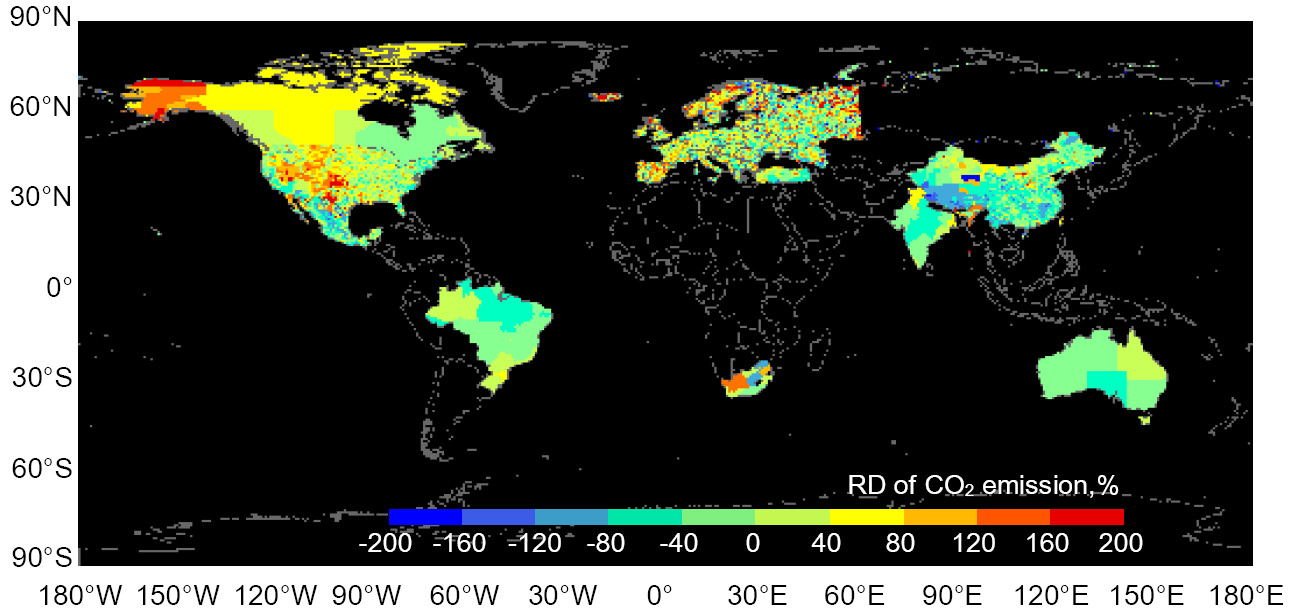
\includegraphics[width=0.8\linewidth]{img/ch3/fig_example.png}  %width控制图片宽度占行宽的比例
    \caption{全球NAT-CO2-2007清单与PKU-CO2-2007比较的空间示意图}         %caption的位置决定了标题出现在图表上方或下方
    \label{fig:fig_example}
\end{figure}

\section{表}

用北大word模板中的表格作为例子,插入表格示例如下:

\begin{table*}[!htbp]
\centering
\caption{室外细菌气溶胶香农-维纳指数(H)和均匀性指数(E)\protect\footnotemark[1]}    %注意脚注命令footnotemark,以及\protect命令,表示修正,使其后的代码被识别为命令而非表格的标签
\label{tab:table_example}
\renewcommand\arraystretch{1.6} %控制表格中的行距
\begin{tabular}{ccccccccccccc}  %c表示设置单元格居中,如果是 l 或 r 则分别为左对齐或右对齐
\Xhline{1.5pt}
\multirow{1}{*}{}   & \multicolumn{4}{c}{\textbf{Stage 1 (>7.1 μm)}}   & \multicolumn{4}{c}{\textbf{Stage 2 (4.8-7.1 μm)}} &  \multicolumn{4}{c}{\textbf{Stage 3 (3.2-4.7 μm)}}    \\  
\cline{2-13}
 &  Con &  Low &  Medium &  High &  Con &  Low &  Medium &  High &  Con &  Low &  Medium &  High  \\
 \hline
\textbf{H} &  \textbf{2.52} &  2.58 &  2.57 &  \textbf{\textit{2.24}} &  \textbf{2.48} &  2.21 &  2.21 &  \textbf{\textit{2.36}} &  \textbf{2.66} &  2.65 &  2.64 &  2.53 \\
\textbf{E} &  0.87 &  0.88 &  0.93 &  0.85 &  0.9 &  0.86 &  0.86 &  0.85 &  0.9 &  0.9 &  0.85 &  0.88 \\ 

\Xhline{1.5pt}
\end{tabular}
\end{table*}

\footnotetext[1]{这里做一个脚注的例子。同时指出,该示例表格宽度超过了行宽,会使得编译时警告,且排版出的表格不够漂亮。使用者如遇类似情况可自行查询LaTex用法,减小宽度、表格居中或页面横置,以使得排版美观。}

\section{问题}

\subsection{交叉引用时的空格问题}

引用图片、数字或公式,都会遇到一个问题,即编号的阿拉伯数字和前后文字距离过近,排版时很不好看,需要手动添加空格或者公式环境下的波浪符号(LaTex会编码为空格)以隔开。例如:图\ref{fig:fig_example}表明、图 \ref{fig:fig_example} 表明、图$~$\ref{fig:fig_example}$~$表明,就可以看出区别。使用者可自行调整。

\subsection{长表格和表格注释}

本人论文写作中遇到两个问题。其一是长表格问题,可以通过\texttt{longtable}环境解决。其二是对表格的某些单元格添加表注,可以通过在表格下方添加注释,或者在页面下方添加脚注的方式解决。这些问题并不复杂,如遇到请使用者自行查询。另,pkuthss v1.9.4模板中有两个问题的例子,可参考其代码。

\subsection{图表位置问题}

查看示例代码可发现,图表位置的设置为\texttt{[!htbp]},意为按照“当前位置、页面顶部、页面底端和另一页搜寻最优位置”四种方式依次选取合适的位置放置图表。但是,排版时可能出现图表位置不美观的情况,使用者可以通过在源代码中调整插入图表代码的位置,或者改变图表位置的设置解决。   
    \chapter{公式}
\label{chap:equation}

本章简要介绍公式使用的方法、问题和技巧。

\section{示例}

LaTex编排公式可以在句中插入公式(例如$1+1=2$),也可以使用\texttt{equation}环境编排公式,使用者需要对LaTex的公式语法有一定的了解。这里给出一个公式的例子\cite{Yao_2015}:
\begin{equation}
\label{eq:Vs_azi_aniso}
    \begin{aligned}
    \hat{\beta}_{\mathrm{SV}} &\approx V_{\mathrm{SV}}\left(1+\frac{G_c}{2L}\cos2\psi+\frac{G_s}{2L}\sin2\psi\right) \\
    &=V_{\mathrm{SV}} \left[ 1+\Lambda_{\mathrm{SV}}\cos2(\psi-\phi_\mathrm{F}) \right]
    \end{aligned}
\end{equation}
公式 \eqref{eq:Vs_azi_aniso} 展示了如何换行、如何对齐、如何使用加大的括号、如何打出约等号等操作。事实上,LaTex对公式的排版有很多技巧,使用者可以根据自己的需求查询相应用法。注意到这里使用\texttt{\string\eqref}引用,而非\texttt{\string\ref}(效果为公式 \ref{eq:Vs_azi_aniso}),前者会自动带括号,但括号是英文字体,后者只有数字,可以自己加中文括号。本人建议是哪个美观用哪个。

\section{问题}

LaTex在公式环境下,中文不一定能正确编译,所以尽量避免用中文。例如一些分段函数,可用“if”、“otherwise”代替“如果”、“其他”等条件。

一些审稿人可能要求独占一行的公式后边也需要加入“,”或者“.”以表示公式也在一句话之中,这一点在北大论文模板中没有提到。本人的建议是如果要用就全部加上,而且加在公式的最后一个字符结束处。如果不用就都不加,因为公式往往会独占一行排列,自动断句,所以公式后有无标点并不影响阅读。

\section{技巧}

许多时候我们需要从已发表的论文中提取公式,转化为LaTex代码,如果全部手打是非常繁琐的。利用图片识别将公式转为代码的工具市面上有不少,这里推荐两个:

\begin{enumerate}[itemindent=0.3em]     % 用enumerate环境可能需要控制缩进量
    \item \texttt{mathpix}:识别公式准确,但有识别数量的免费限额,可能要收费使用。下载地址:https://mathpix.com/。
    \item \texttt{simpletex}:识别公式基本准确,对“粗体”、“正体”等的识别相对较差(例如$x$、$\mathrm{x}$、$\mathbf{x}$),需手动调整,但免费。下载地址:https://simpletex.cn/。
\end{enumerate}
    
    \chapter{问题及思考}
\label{chap:problem}

本模板存在一些问题,这些问题对论文写作可能影响没有那么大,但终究不够完美。本人通过一些不那么“美”的方式进行了解决,期待使用者找到更好的解决方案。

\section{封面问题}

封面存在两个问题,其一是模板默认标题有两行下划线,不论标题几行,下划线都是两行。其二是自2024年始,封面中加入了“学术学位”和“专业学位”的选项,该模板并没有。

推荐的解决方法:封面用学校提供的word文档编辑,转为pdf格式,然后用pdf编辑软件替换本模板的封面。或者用pkuthss v1.9.4模板,已解决该问题。

\section{目录问题}

本模板没有找到合适的将“目录”放在目录里的方法,因此目录里没有“目录”一项。另外,为了将“摘要”和“ABSTRACT”放入目录,在\texttt{abs.tex}中使用了 \texttt{\string\addcontentsline\{toc\}\{chapter\}\{摘要\}} 命令,使得编译后的pdf文档在书签侧栏可能出现两个“摘要”和“ABSTRACT”,手动删去一个即可。

此外,本模板也提供了插入图、表索引的选择,在\texttt{main.tex}中可选。请注意,图表索引是将图表的\texttt{\string\caption}中的文字全部加入目录,因此图注中有较多说明文字时(比如红线代表了xxx,蓝色三角形代表了xxx),不适宜插入图表索引。

\section{字体问题}

本模板是基于pkuthss v1.9.2开发的,该模板默认字体是\texttt{fandol},并非宋体。其优点是免费使用,overleaf支持,且和宋体几乎无差;其缺点是字体库较少,对一些生僻字可能无法显示。比如本人姓名中的“吉吉”(zhe2),是无法显示的。由于本人的论文中没有用生僻字,所以只有在封面和个人简历中可能出现姓名显示不完全。对此,本人的做法是在编译后的pdf文档中修改。

本人测试发现,在windows环境下,配置好本地环境,使用VSCode编译,设置\texttt{fontset=windows},生僻字问题可以解决,且字体也和宋体几乎无差。

目前最新版的pkuthss v1.9.4支持了宋体,有兴趣的同学可以使用该版本试一试。但该模板代码风格和v1.9.2版本有些区别,并不能直接移植过去,使用者可对比选择。

\section{段落间距问题}

使用word排版论文时,段落间距一般和行间距是一样的。但使用本模板在排版时,有时会遇到段落间距比行间距更大的情况,使段间空行比较突出。比如一页的最后出现章节标题之时,为了使章节标题不会出现在本页最后一行,该模板在排版时会倾向于将本页其他段落段间距加大,让章节标题排在下一页。又或者,正常排版时,下一页的第一行是一个公式,那么该模板会让本页的段间距加大,从而让一些文字被“挤”到下一页,避免下页第一行是公式。

这个问题遇到了自然明白,一般论文写作不会出现大篇幅的段间距过大,即便有几页如此,也并不显得不美观,因此本人并未对此进行任何修正。在致谢部分(见\texttt{ack.tex}),有添加\texttt{\string\setlength\{\string\parskip\}\{0pt\}}的代码禁止段间距离拉长,使用者可以注释掉这行代码查看该问题的效果。

\section{论文补充页面的插入}

提交最终版论文一般需要插入版权声明、原创性声明等等页面。在本模板中,插入“版权声明”(见\texttt{copy.tex})和“北京大学学位论文原创性声明和使用授权说明”页面(见\texttt{origin.tex})是通过插入图片的方式实现的。然而,从个人门户下载的pdf文件并不能直接插入,可以将这些文件先用Adobe Illustrator打开,再另存为pdf文件,使其变为矢量图,就可以插入了。当然,也可以在写作时不添加这些页面,最终版论文插入这些文件的扫描件即可。

\section{其他问题}

北大未名bbs论坛反映了pkuthss v1.9.2的一些其他问题,比如一些数学符号字体不正确等,本人并未遇到。如有任何问题可在bbs上提问和讨论。
    \chapter{总结和展望}
\label{chap:conclusion}

\section{总结与创新性}

本研究xxx

本研究的主要创新性是xxx

\section{展望}

基于本研究,提出以下展望,xxx


    
    \appendix
    \chapter{附录示例1}

\section*{A1\ \ 标题1}

\section*{A2\ \ 标题2}

\chapter{附录示例2}

    \printbibliography[heading = bibintoc]
    % 如有需要使用研究生成果页
    \chapter*{个人简历、在学期间科研成果与荣誉}
\markboth{个人简历、在学期间科研成果与荣誉}{}
\phantomsection
\addcontentsline{toc}{chapter}{个人简历、在学期间科研成果与荣誉}

\subsection*{\bfseries 个人简历}

何年何月出生何地

何年何月何地本科

何年何月何地博士,导师

\subsection*{\bfseries 发表论文}

\setlength{\parskip}{6pt}
\renewcommand\labelenumi{[\theenumi]}

\begin{enumerate}
  \item \textbf{Mr. ZYZ}, others. (2024). Paper name. \textit{Journal name, 1}, 001-010. %\url{https://doi.org/xxxx}
  \item \textbf{Mr. ZYZ}, others. (2024). Paper name. \textit{Journal name, 1}, 001-010. %\url{https://doi.org/xxxx}
\end{enumerate}

\subsection*{\bfseries 参加学术会议}
\setlength{\parskip}{6pt}
\renewcommand\labelenumi{[\theenumi]}

\begin{enumerate}

    \item \textbf{Mr. ZYZ}, others. Presentation name. Dec. 2023, \textit{AGU Fall Meeting 2023}, San Francisco, USA, Oral presentation.

\end{enumerate}

\subsection*{\bfseries 获得荣誉}
\setlength{\parskip}{6pt}
\renewcommand\labelenumi{[\theenumi]}

\begin{enumerate}

  \item 奖项1,2019年12月,2021年12月
  \item 奖项2,2023年12月
\end{enumerate}

\subsection*{\bfseries 其他项目}
\setlength{\parskip}{6pt}
\renewcommand\labelenumi{[\theenumi]}

可以根据需要添加,例如科研项目、野外工作、专利、软件、学术服务(比如审稿人)等等。



   \backmatter
   \chapter{致谢}
\setlength{\parskip}{0pt}

感谢pkuthss的开发者和维护者们,感谢工学院模板的开发者。感谢为本人论文写作提出各种意见和建议的老师及同学。

另外,本模板的学号“4367497427”是个小彩蛋,设计出来很巧是个十位数,与学号相同,便添加在学号栏,留给使用者探索其含义吧!(这个小彩蛋和本模板的初衷——为地物专业的同学服务——有关)。

    % 需替换门户原创页pdf/扫描pdf
   % Copyright (c) 2008-2009 solvethis
% Copyright (c) 2010-2017,2021 Casper Ti. Vector
% Copyright (c) 2021 Kurapica
% Copyright (c) 2021 iofu728
% All rights reserved.
%
% Redistribution and use in source and binary forms, with or without
% modification, are permitted provided that the following conditions are
% met:
%
% * Redistributions of source code must retain the above copyright notice,
%   this list of conditions and the following disclaimer.
% * Redistributions in binary form must reproduce the above copyright
%   notice, this list of conditions and the following disclaimer in the
%   documentation and/or other materials provided with the distribution.
% * Neither the name of Peking University nor the names of its contributors
%   may be used to endorse or promote products derived from this software
%   without specific prior written permission.
%
% THIS SOFTWARE IS PROVIDED BY THE COPYRIGHT HOLDERS AND CONTRIBUTORS "AS
% IS" AND ANY EXPRESS OR IMPLIED WARRANTIES, INCLUDING, BUT NOT LIMITED TO,
% THE IMPLIED WARRANTIES OF MERCHANTABILITY AND FITNESS FOR A PARTICULAR
% PURPOSE ARE DISCLAIMED. IN NO EVENT SHALL THE COPYRIGHT HOLDER OR
% CONTRIBUTORS BE LIABLE FOR ANY DIRECT, INDIRECT, INCIDENTAL, SPECIAL,
% EXEMPLARY, OR CONSEQUENTIAL DAMAGES (INCLUDING, BUT NOT LIMITED TO,
% PROCUREMENT OF SUBSTITUTE GOODS OR SERVICES; LOSS OF USE, DATA, OR
% PROFITS; OR BUSINESS INTERRUPTION) HOWEVER CAUSED AND ON ANY THEORY OF
% LIABILITY, WHETHER IN CONTRACT, STRICT LIABILITY, OR TORT (INCLUDING
% NEGLIGENCE OR OTHERWISE) ARISING IN ANY WAY OUT OF THE USE OF THIS
% SOFTWARE, EVEN IF ADVISED OF THE POSSIBILITY OF SUCH DAMAGE.

{
	\ctexset{section = {
		format+ = {\centering}, beforeskip = {40bp}, afterskip = {15bp}
	}}
	\specialchap{北京大学学位论文原创性声明和使用授权说明}

	% 学校书面要求本页面不要页码,但在给出的 Word 模版中又有页码。
	% 此处以学校书面要求为准。
	\thispagestyle{empty}
	
	% 替换扫描pdf,去除includegraphics前注释
	\begin{textblock}{1}(-0.8,-0.08)
		\colorbox{white}{
			
\includegraphics[height = 1.2448\textheight]{img/lwsm_example.pdf}
		}
	\end{textblock}
}

% vim:ts=4:sw=4
 
\end{document}

% vim:ts=4:sw=4